\documentclass{standalone}

\usepackage{tikz}
\usetikzlibrary{positioning}
\usepackage{pgfplots}
\pgfplotsset{compat=1.12}

\begin{document}

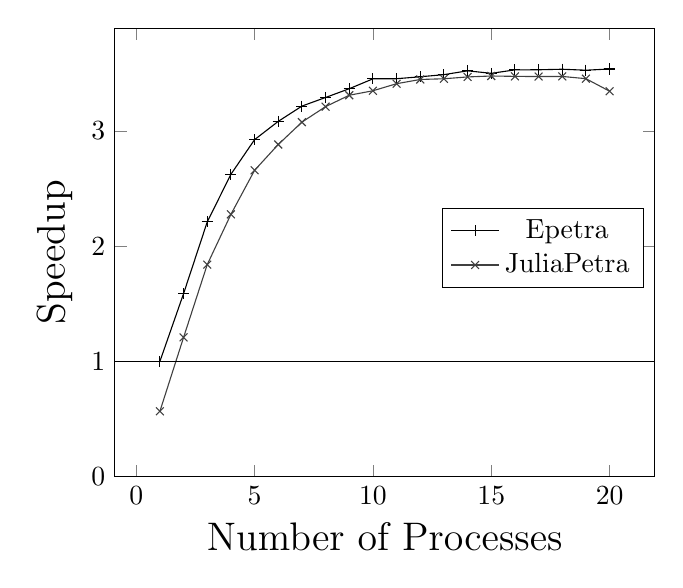
\begin{tikzpicture}
	\begin{axis}[
		xlabel = {\Large Number of Processes},
		ylabel style = {align=center},
		ylabel = {\Large Speedup},
		ymin = 0,
		legend style={at={(0.98,0.6)}}
	]
		\addplot[color=black,mark=+] coordinates{(1, 1) (2, 1.5883416) (3, 2.210738) (4,2.6240833) (5, 2.924896) (6,3.083557) (7, 3.216142) (8,3.290998) (9,3.36702) (10, 3.452862) (11,3.45405) (12,3.470708) (13,3.489314) (14,3.52233) (15, 3.500694) (16,3.53057) (17,3.53162) (18,3.536203) (19, 3.5278034) (20, 3.538395)};
		\addlegendentry{Epetra}
		\addplot[color=darkgray,mark=x] coordinates{(1, 0.5667807) (2, 1.208247) (3, 1.8400692) (4,2.276446) (5, 2.658824) (6,2.882781) (7, 3.0769025) (8,3.21155) (9,3.31040) (10, 3.349281) (11,3.410606) (12,3.447333) (13,3.453482) (14,3.4693506) (15, 3.4774509) (16,3.474327) (17,3.472608) (18,3.473677) (19, 3.4541359) (20, 3.345339)};
		\addlegendentry{JuliaPetra}
		\draw (axis cs:-1,1) -- (axis cs:25,1);
	\end{axis}
\end{tikzpicture}

\end{document}